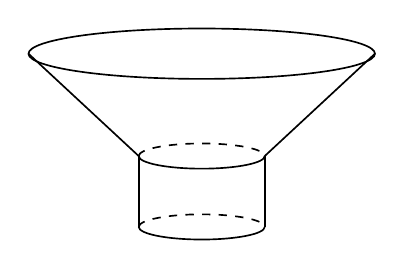
\begin{tikzpicture}[x=1cm,y=1cm,line width=.6pt,font=\normalsize]
% top cone rim (wide ellipse)
\draw (0,2.2) ellipse (2.2 and 0.32);
% cone sides to narrow neck
\draw (-2.2,2.2) -- (-0.8,0.9);
\draw (2.2,2.2) -- (0.8,0.9);
% neck (cylinder top): front solid, back dashed
\draw (-0.8,0.9) arc (180:360:0.8 and 0.16);
\draw[dashed] (-0.8,0.9) arc (180:0:0.8 and 0.16);
% cylinder sides
\draw (-0.8,0.9) -- (-0.8,0);
\draw (0.8,0.9) -- (0.8,0);
% cylinder bottom: front solid, back dashed
\draw (-0.8,0) arc (180:360:0.8 and 0.16);
\draw[dashed] (-0.8,0) arc (180:0:0.8 and 0.16);
\end{tikzpicture}
